\subsection{XY-Wing}
Die Technik \textit{XY-Wing} wird manchmal auch nur \textit{Y-Wing} genannt, da sie aussieht wie ein \textit{X-Wing} (siehe Kapitel \ref{X-Wing}) nur mit drei Ecken. Zuerst sucht man eine Zelle, in der nur noch 2 Kandidaten verblieben sind. Diese Kandidaten nennt man dann x und y. Daher kommt der im Allgemeinen bekanntere Name der Strategie. Im nächsten Schritt sucht man nun eine Zelle, die in einer gemeinsamen Figur mit der ersten Zelle liegt und auch nur noch 2 Kanididaten der Form hat, dass einer der Kandidaten dem x aus der ersten Zelle entspricht und der zweite Kandidat ungleich dem y ist. dieser wird nun z genannt. Anschließend sucht man eine dritte Zelle mit nur noch zwei verbliebenen Kandidaten, die ebenfalls in einer gemeinsamen Figur mit der ersten Zelle liegt, aber nicht in der selben wie die zweite gefundene Zelle. Wenn diese Zelle nun die Kandidaten y und z enthält, dann hat man einen \textit{XY-Wing} gefunden. Gelöscht werden kann nun der Kandidat z aus der Zelle, die von der zweiten und dritten Zelle ausgeschlossen wird. Das funktioniert, da in der ersten Zelle entweder x oder y steht. Wenn in der ersten Zelle x steht, dann steht in der zweiten Zelle z, da dort nur x und z stehen kann, x aber durch die erste Zelle ausgeschlossen wird. Wenn in der ersten Zelle aber y steht, dann muss in der dritten Zelle z stehen, da dort nur y und z stehen können und y ausgeschlossen wird. Daher steht in einer der beiden Zellen z und alle Kandidaten von z, die durch beide Felder ausgeschlossen werden, können gelöscht werden.

\begin{figure}[h]
\begin{center}
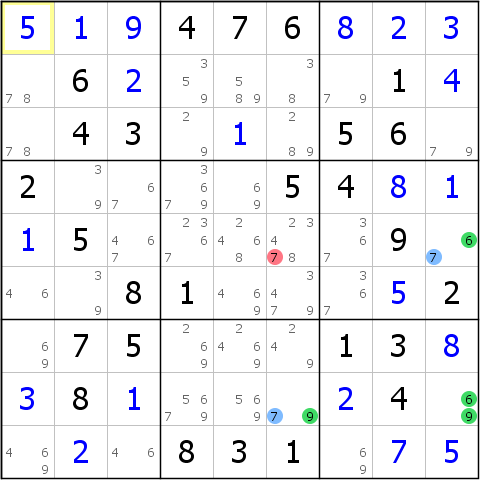
\includegraphics{./img/XY_Wing.png}
\caption{XY-Wing}
\end{center}
\end{figure}

In der obigen \textbf{Abbildung 3.13} stehen in z1s3 die Kandidaten 5 für x und 7 für x. In Zelle z1s6 stehen 5 für x und 2 für z. in z2s1 stehen 7 für y und 2 für z. Wenn in z1s3 die Ziffer 5 steht, dann muss in z1s6 die Ziffer 2 stehen und den Kanididaten 2 in z2s6 ausschließen. Wenn in z1s3 die Ziffer 7 steht, dann steht in z2s1 die Ziffer 2 und schließt ebenfalls die Ziffer 2 in z2s6 aus. Somit kann diese dort in keinem der beiden Fälle stehen und kann gelöscht werden.